\chapter{实验做好之后...}
\begin{introduction}
    \item 把 xv6 跑在国产硬件上
    \item 给 xv6 增加一个应用编程语言
    \item 更多好玩的计划
\end{introduction}

完成了全部的 xv6 实验后, xv6 作为现代体系结构上对 Unix v6 的一次复刻,其可玩性不只于 6.S081 提供的实验题目。下面笔者进行了两个额外的有趣的关于 xv6-riscv 的实验,供读者参考。

\section{把 xv6 跑在国产硬件上}

\subsection{Lichee RV 开发板概览}

虽然 RISC-V 架构仍然没有成熟的商业产品,但我国仍然有一些公司致力于开拓计算机系统结构的最新领域,并且产出了很好的成品。

今年年初,有一款国产 RISC-V 开发版凭借其极其低廉的价格迅速占据了市场,即 Lichee RV - Nezha CM \footnote{Lichee RV - Nezha CM \url{https://wiki.sipeed.com/hardware/zh/lichee/RV/RV.html}} 。该开发板使用的CPU是全志D1,其是一块基于阿里平头哥玄铁 C906 IP核的微处理器,兼容 RISC-V 的 RV64IMAC 指令集,拥有 512MB 的 DDR3 内存,并有可用的 MMU 提供对操作系统的支持。该开发板 CPU 的功能如下图所示:

\begin{figure}[H]
  \centering
  \includegraphics[width=0.5\textwidth]{c906.png}
  \caption{ C906 结构概览 }
\end{figure}

关于 C906 的文档可以在阿里平头哥的GitHub库里找到\footnote{参见:\url{https://github.com/T-head-Semi/openc906/tree/main/doc}},但对于 Lichee RV 开发板,由于一些商业上知识产权的原因,该开发板的很多外设的驱动都是不公开的;但幸运的是,运行 xv6 所需要的 uart 驱动是可用的,故而笔者在查阅了众多资料后,自费入手了一块 Lichee RV ,企图将 xv6 移植到其上并成功通过 \lstinline{usertests} 。

笔者购得的 Lichee RV 如下图所示:

\begin{figure}[H]
  \centering
  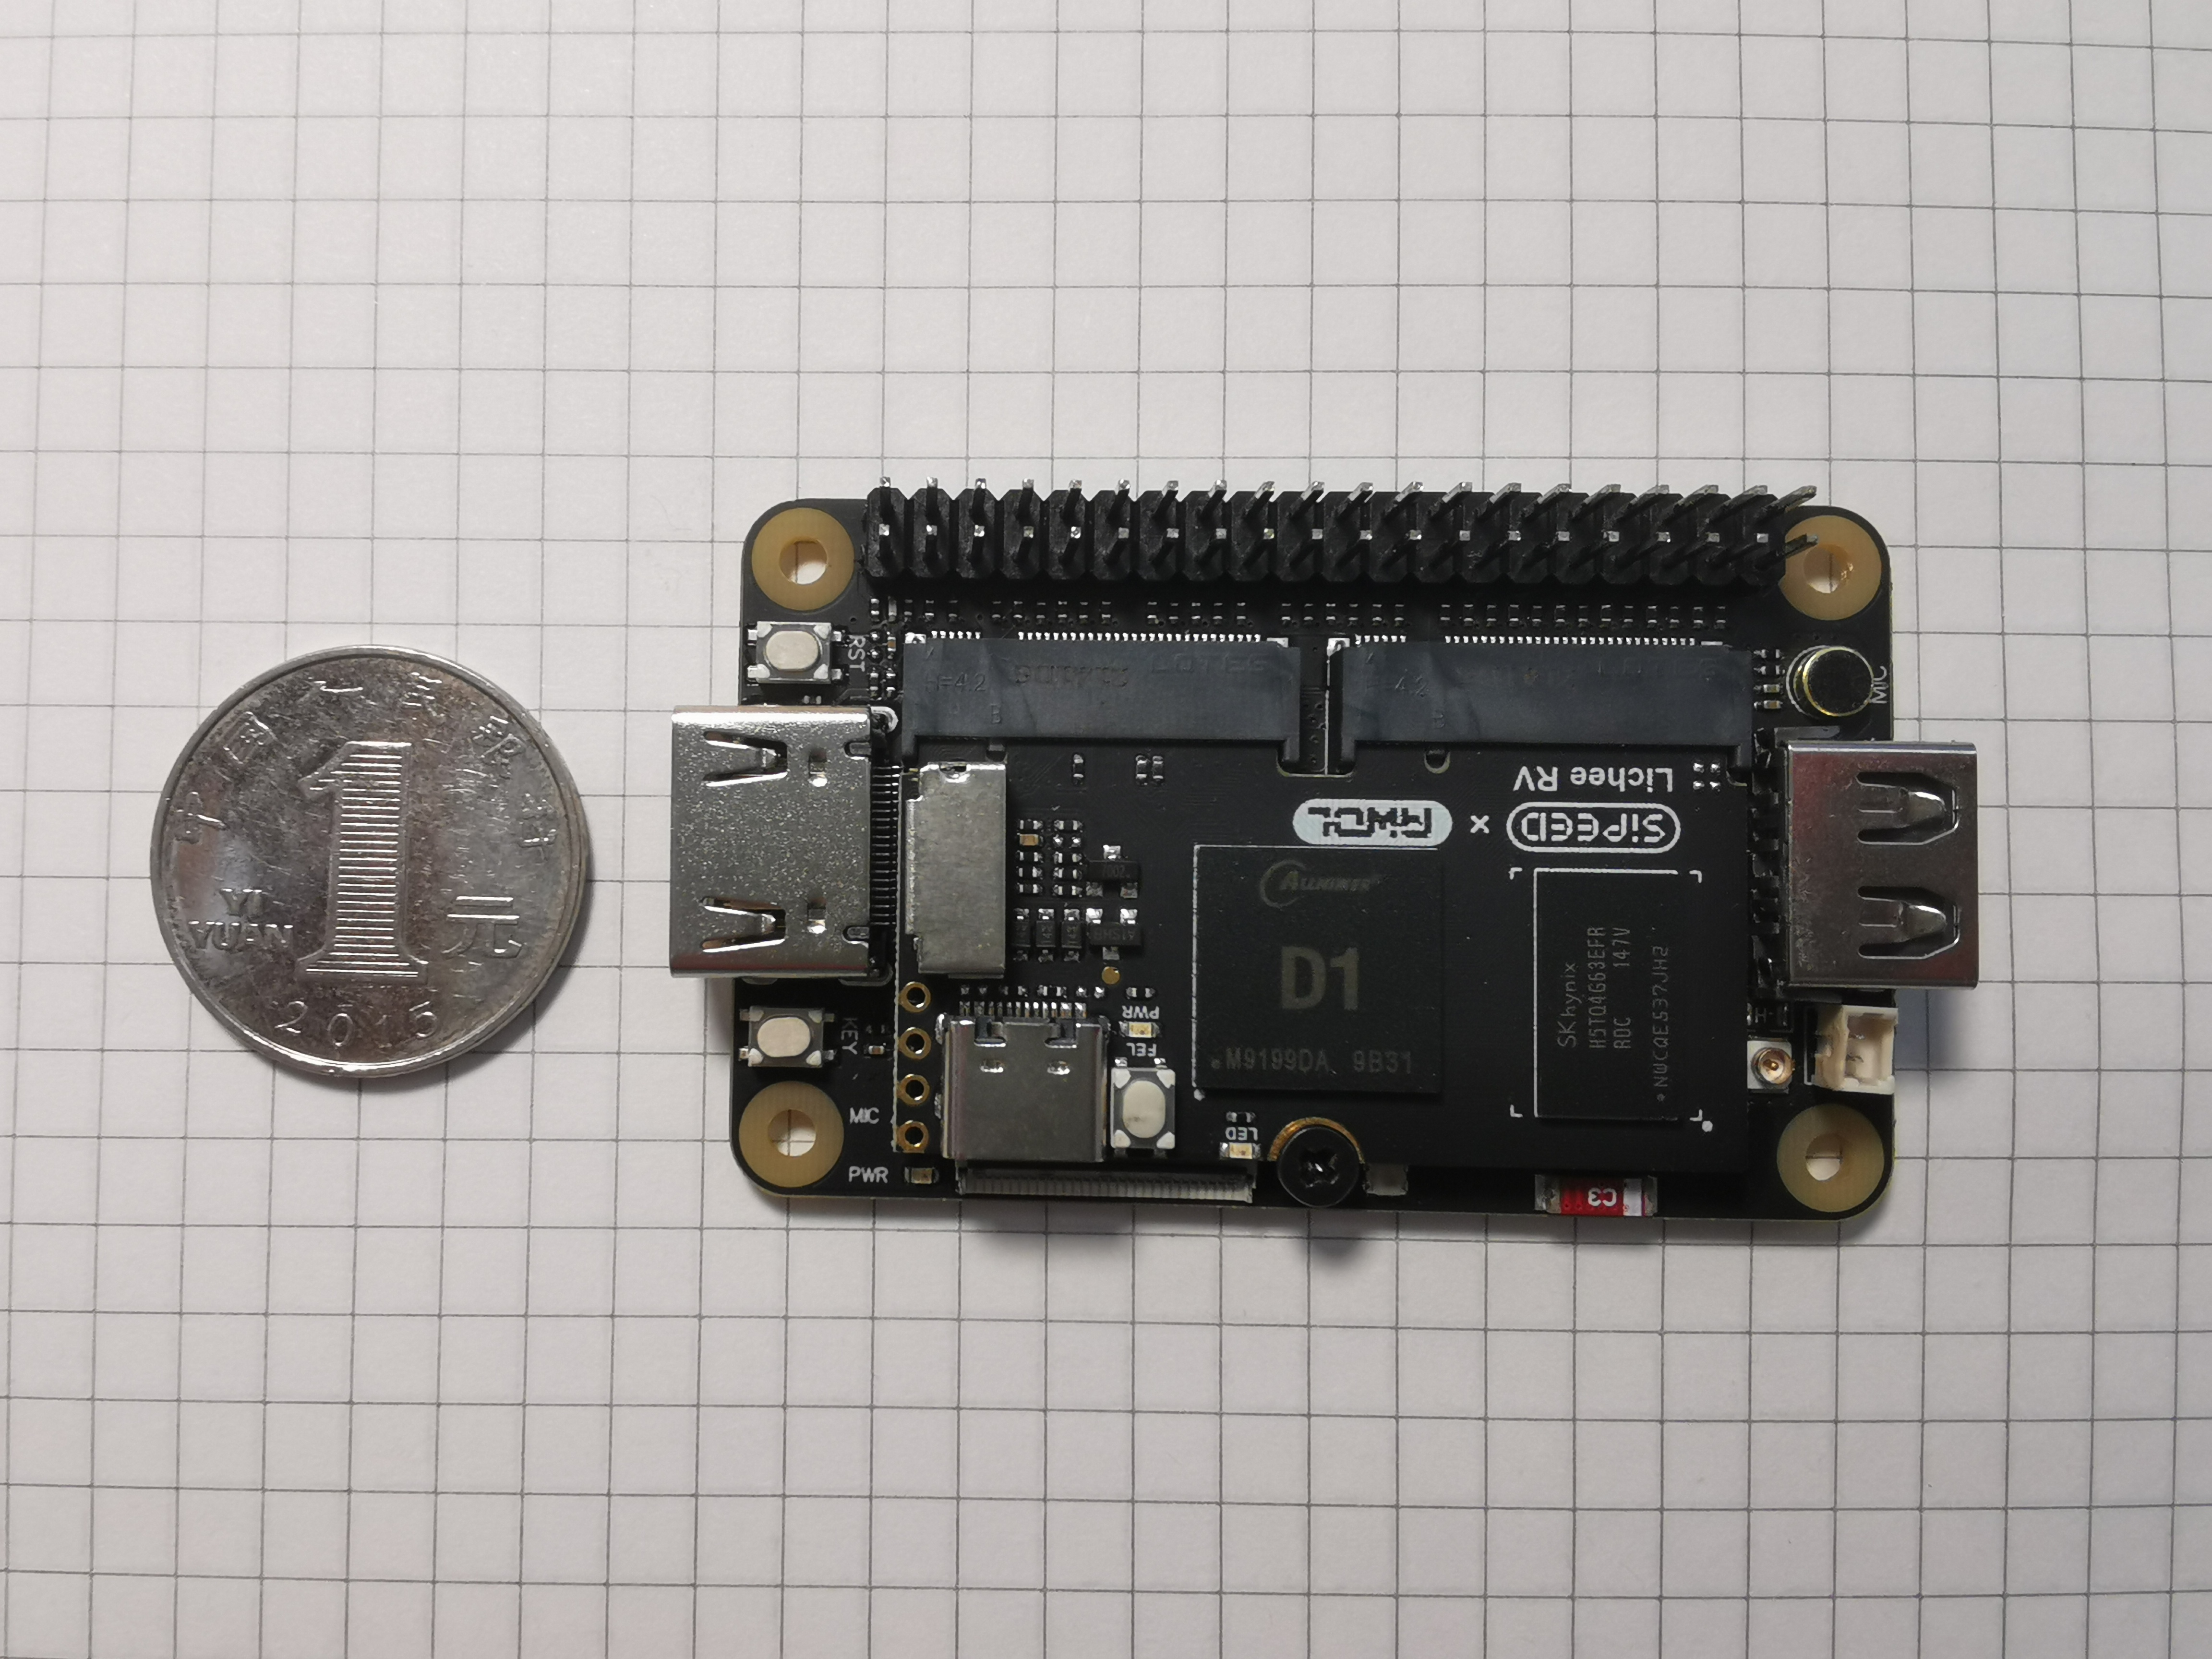
\includegraphics[width=0.7\textwidth]{LC_RV.jpg}
  \caption{ 笔者的 Lichee RV 开发板 }
\end{figure}

\subsection{前期准备}

在开始移植前,我们需要准备一份干净的 xv6-riscv 代码库,在终端中执行 \lstinline{git clone git://github.com/mit-pdos/xv6-riscv.git} 将代码库克隆到本地。

然后,我们需要从GitHub上下载用于调试开发板的工具 \lstinline{xfel} \footnote{\url{https://github.com/xboot/xfel}} 用于将我们移植好的 xv6 内核加载到开发板内存中并开始执行。之后需要准备串口通信软件,笔者使用的是 Putty。

\begin{theorem}[在 Windows 系统上使用 \lstinline{xfel}]
    在 Windows 系统上使用 \lstinline{xfel} 还需要安装 \lstinline{zadig-2.7.exe} 驱动,才能正常使用。Windows 平台驱动和预编译的 \lstinline{xfel} 程序可以在 \url{https://github.com/xboot/xfel/releases/download/v1.2.9/xfel-windows-v1.2.9.7z} 下载。
\end{theorem}

除了软件和开发板以外。我们还需要准备一根 USB C-type 线用于通过 \lstinline{xfel} 刷写开发板,以及一块诸如 CH341 的 USB 转串口的设备,用于通过 uart 与开发板进行通信。当然,几根杜邦线也是必不可少的,(除了一台PC机外)全部需要用到的设备如下图所示:

\begin{figure}[H]
  \centering
  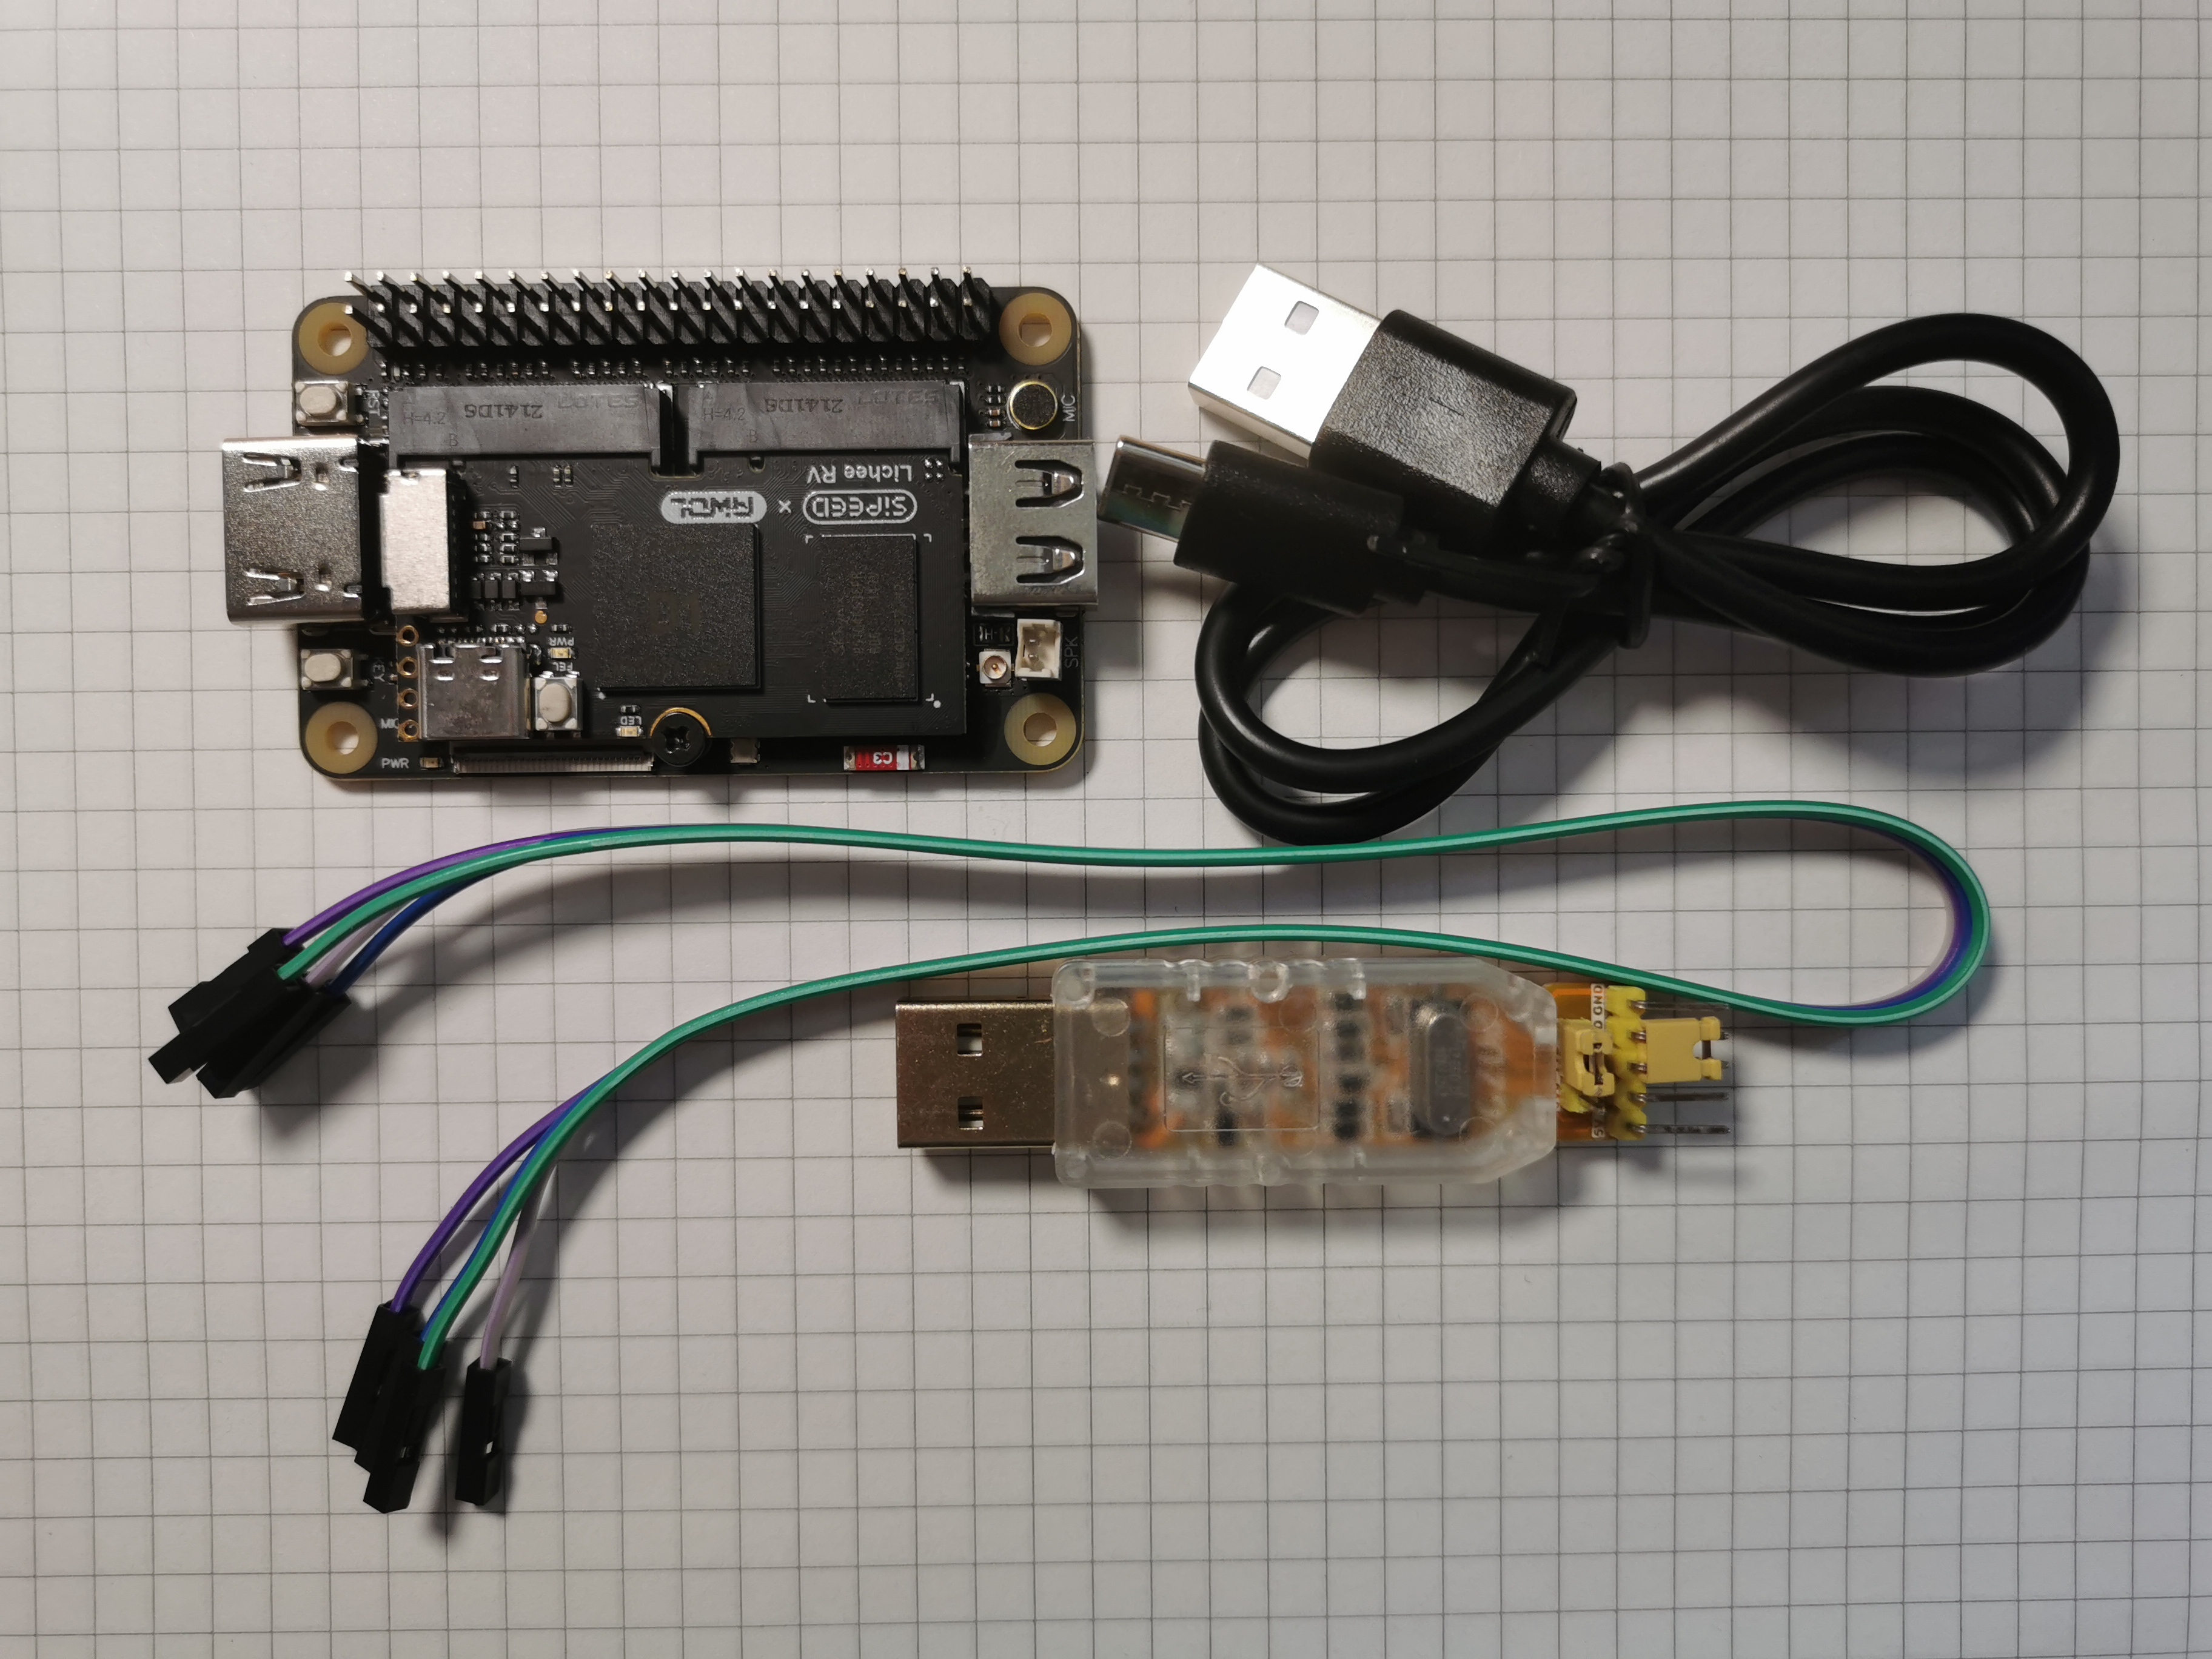
\includegraphics[width=0.7\textwidth]{RV_Kit.jpg}
  \caption{ 需要用到的硬件设备 }
\end{figure}

准备好这些设备后,使用 USB C 线将开发板连接到电脑,然后按一下开发板上的 fel 按钮, fel 按钮的位置在下图绿色LED灯上方的红框中:

\begin{figure}[H]
    \centering
    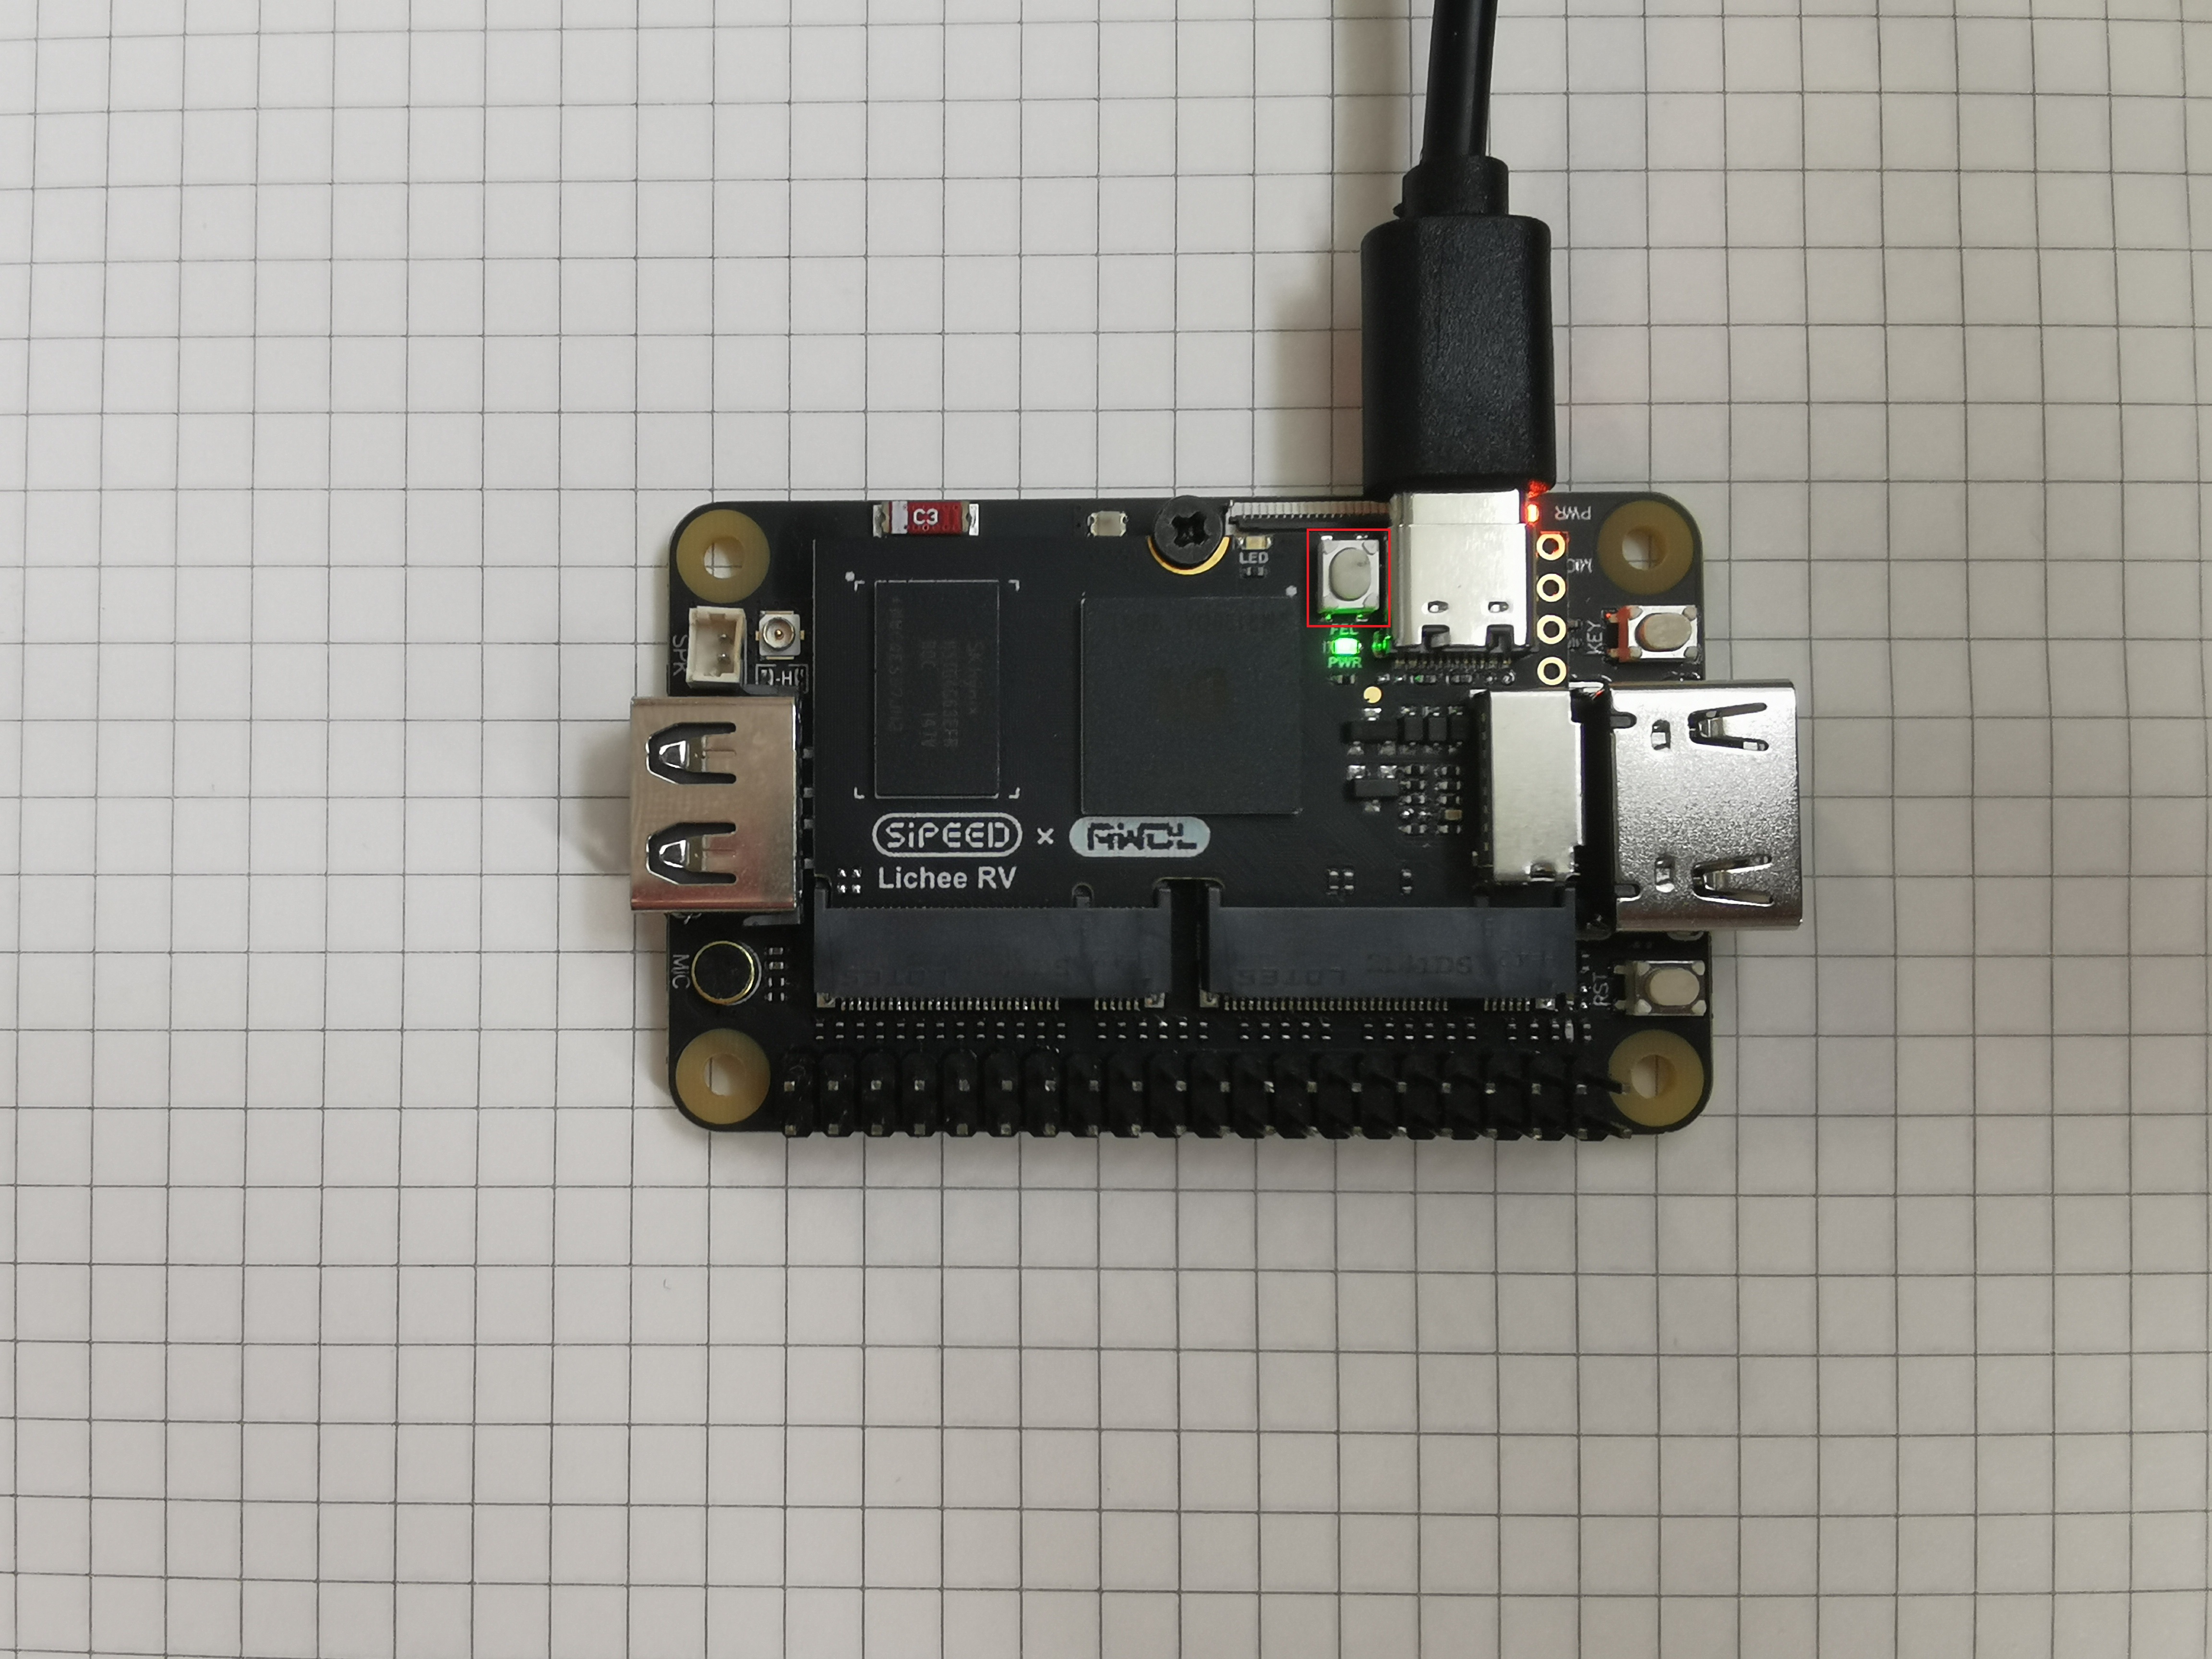
\includegraphics[width=0.8\textwidth]{RV_xfel1.jpg}
    \caption{ 测试开发板与 \lstinline{xfel} 的配置(1) }
\end{figure}

然后在终端中执行 \lstinline{xfel version} ,若出现类似下图所示的结果,即为 \lstinline{xfel} 正确识别开发板,开发板与 \lstinline{xfel} 的配置正确:
\begin{figure}[H]
    \centering
    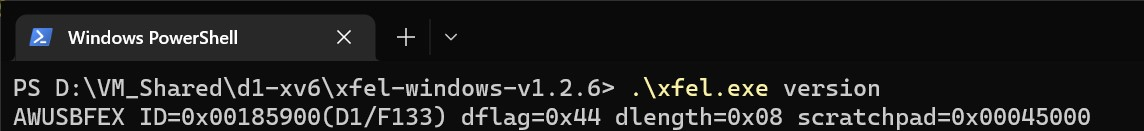
\includegraphics[width=0.7\textwidth]{RV_xfel2.jpg}
    \caption{ 测试开发板与 \lstinline{xfel} 的配置(2) }
\end{figure}

如果无法识别,则需要重新按下开发板上的 fel 按钮。由于不同批次的硬件的差异,上述结果可能略有不同,但大致上都会有诸如 \lstinline{D1/F133} 之类的字样出现。

\subsection{修改 xv6 代码}
这里大致说明一下修改代码的步骤,具体与原版 xv6 的不同点可以查看 \href{https://github.com/jwyjohn/xv6-riscv/commit/54745c4f7eea4af81f8e044953119ad81cd6822b#diff-c53dc675dd68c013f3e29c34d517877d7da3a48af39fe77b7b9541751aed722c}{这个diff} 的结果。

1. 将 xv6 移植到真实的硬件上时,第一个遇到的问题就是硬件的初始化问题。好在初始化时钟和硬件的代码已经有人写好\footnote{见 \url{https://github.com/bigmagic123/d1-nezha-baremeta}},我们拿来后(主要是 \lstinline{clk.c} 和 \lstinline{uartinit.c})略作修改就可以放入 xv6 的源码库中。

2. 为适配 Lichee RV,原来的 CLINT, PLIC, UART, UART IRQ 的地址按需修改,并且需要修改链接器脚本 \lstinline{kernel.ld} 使得内核的开始地址改为 \lstinline{0x40000000} 。

3. 由于 D1 具有物理内存保护机制(Physical Memory Protection (PMP)),相比于 qemu 虚拟机而言,需要初始化 PMP 才能成功地从 M 态切换到 S 态。

4. 由于该开发板的公司没有开源的 SD 卡驱动,故而我们使用内存盘模拟硬盘,而非使用 qemu 的 \lstinline{virtio}。

5. 对应的 Makefile 等配置也进行了修改,以方便将 \lstinline{fs.img} 链接入二进制的 \lstinline{kernel}。

\subsection{在开发板上启动 xv6 }

首先,使用 CH341 通过杜邦线连接到开发板的uart针脚,如下图所示:

\begin{figure}[H]
    \centering
    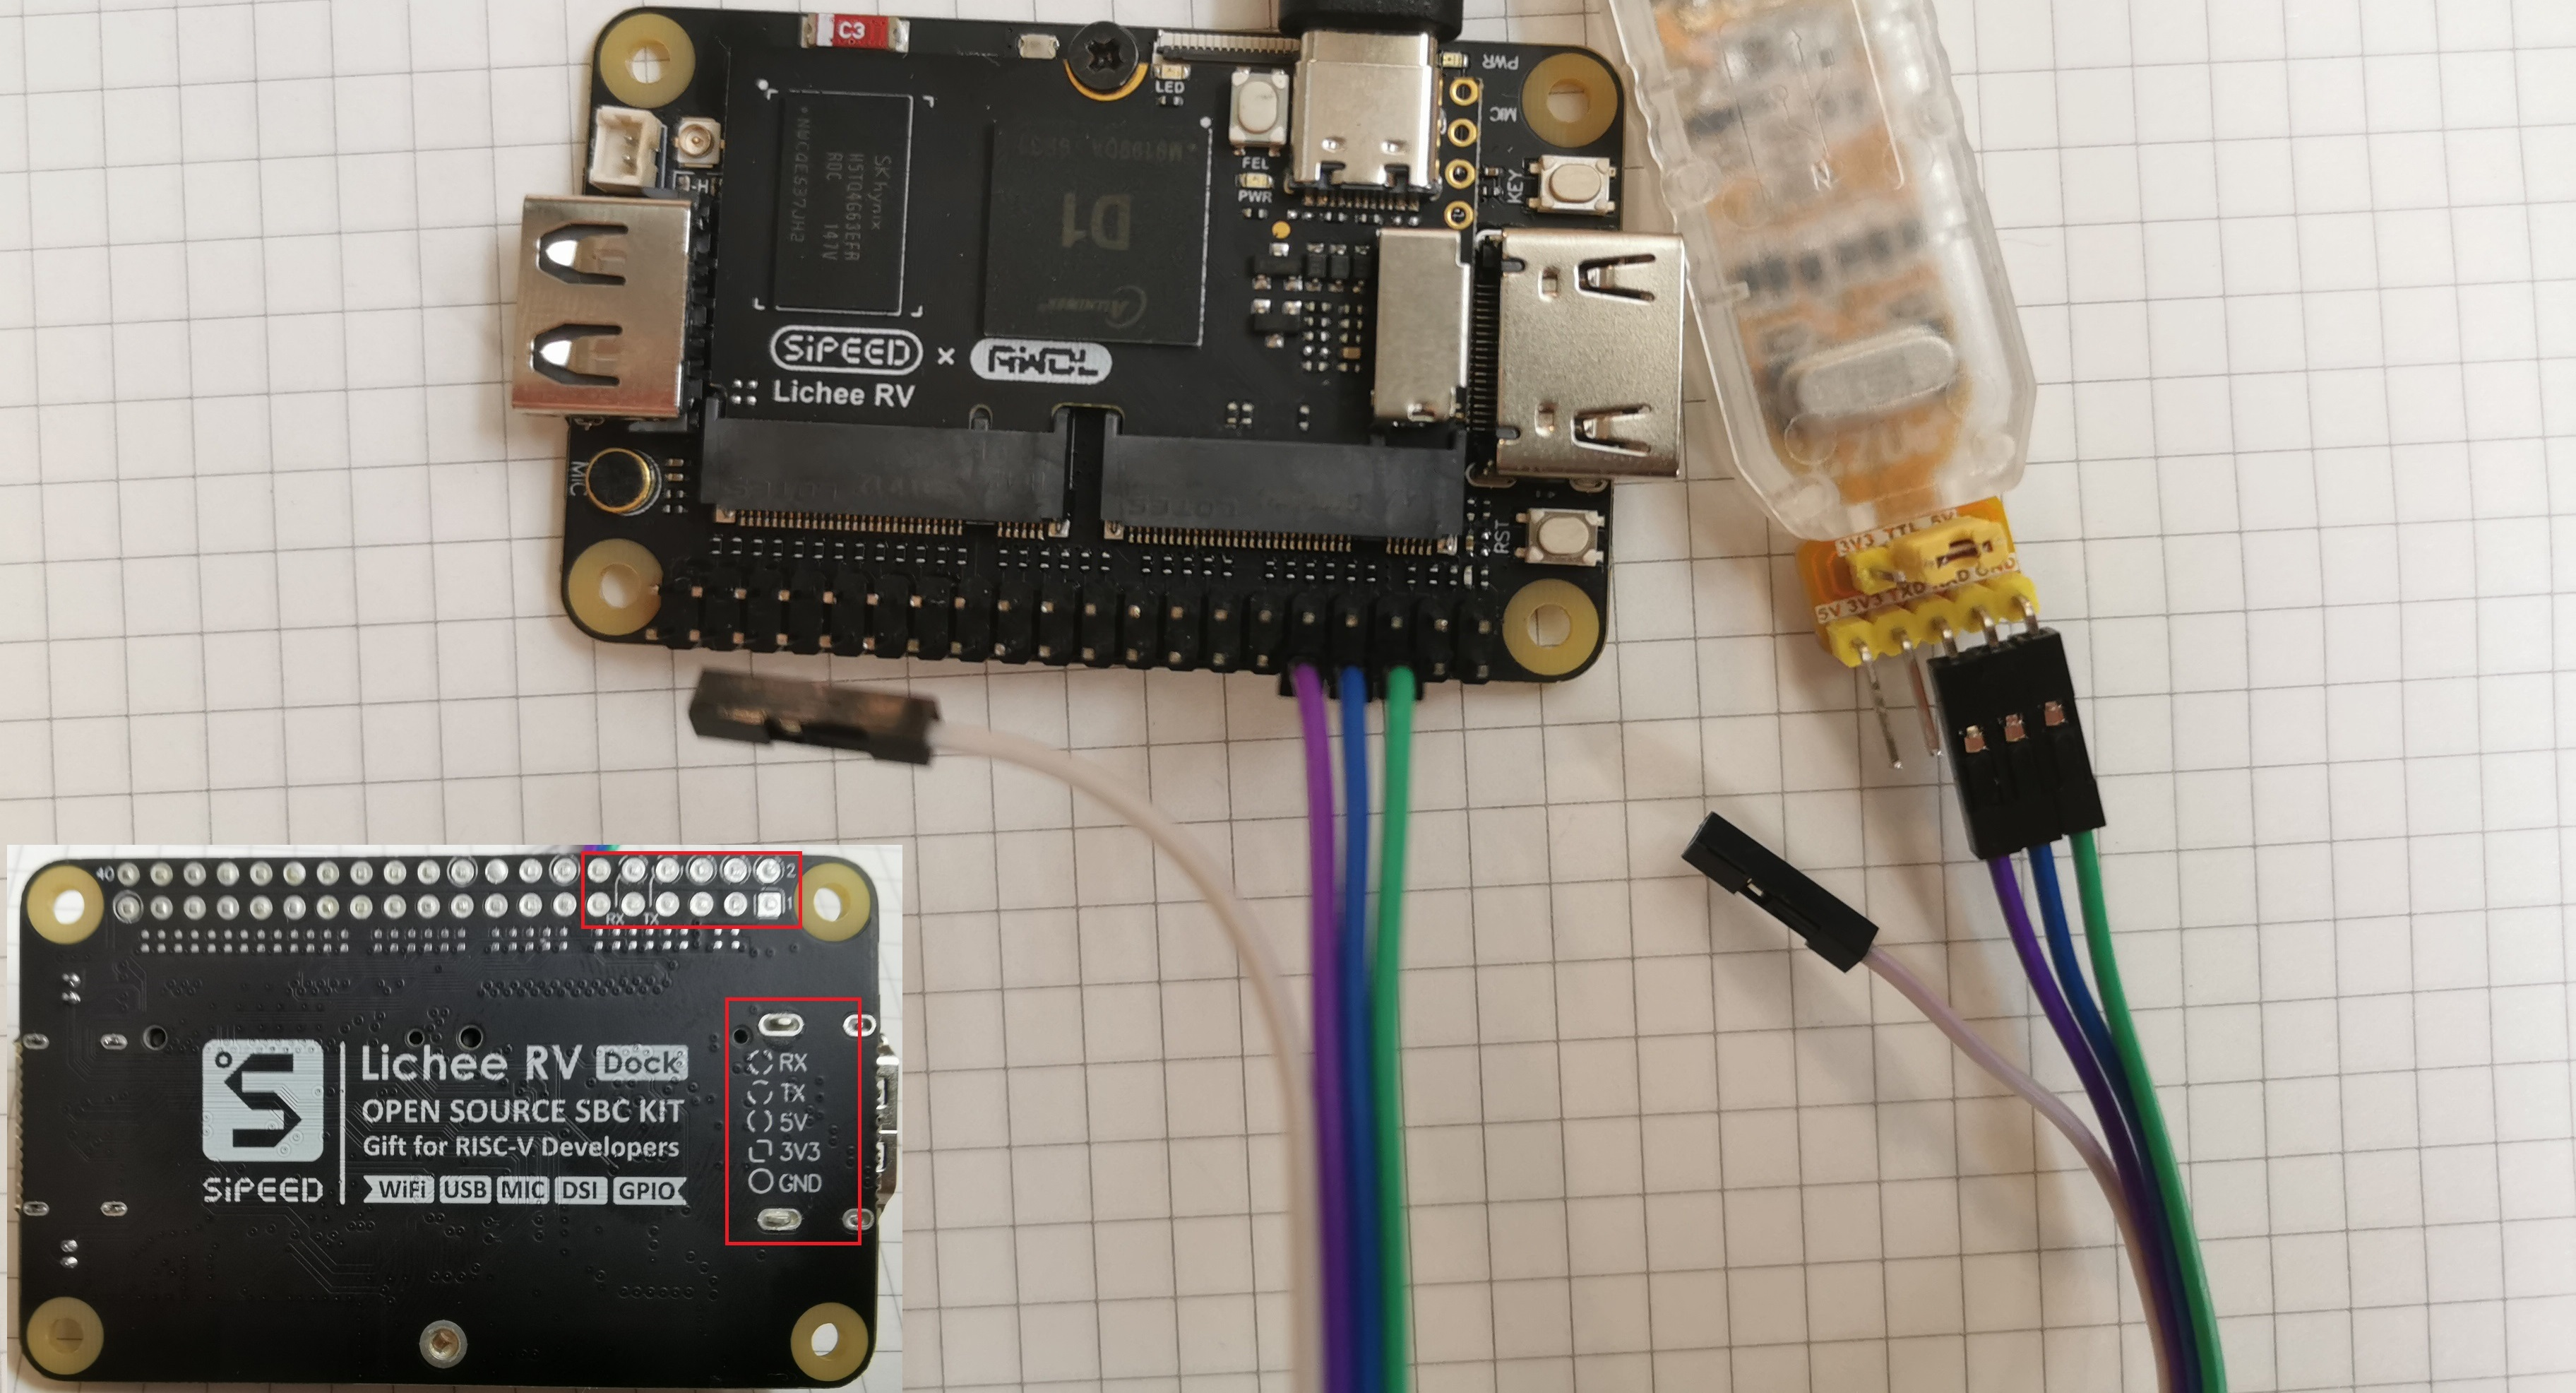
\includegraphics[width=0.7\textwidth]{RV_uart.jpg}
    \caption{ 开发板连接 uart 的线序(见左下红框中图示)}
\end{figure}

然后编译 xv6 的内核镜像,使用 \lstinline{make fs.img && make},成功后生成二进制文件 \lstinline{kernel/kernel.bin},将该文件拷贝到 \lstinline{xfel} 的目录下。

完成编译后,使用 USB C 线将开发板连接到电脑,然后按一下开发板上的 fel 按钮,然后再将接有杜邦线的 CH341 连接至电脑。

此时在终端中执行 \lstinline{xfel version} 确认开发板连接无误;然后在终端中执行 \lstinline{xfel ddr d1} 用于初始化开发板的内存控制器;然后使用 \lstinline{xfel write 0x40000000 ./kernel.bin} 将编译好的内核拷贝到内存中。

此时打开 Putty (或其它串口终端工具),设置波特率为 115200 ,然后打开 CH341 对应的 COM 口。最后在(原来执行xfel的)终端中执行 \lstinline{xfel exec 0x40000000},即可在 Putty 中看到 xv6 的启动信息,过程如下图所示:

\begin{figure}[H]
    \centering
    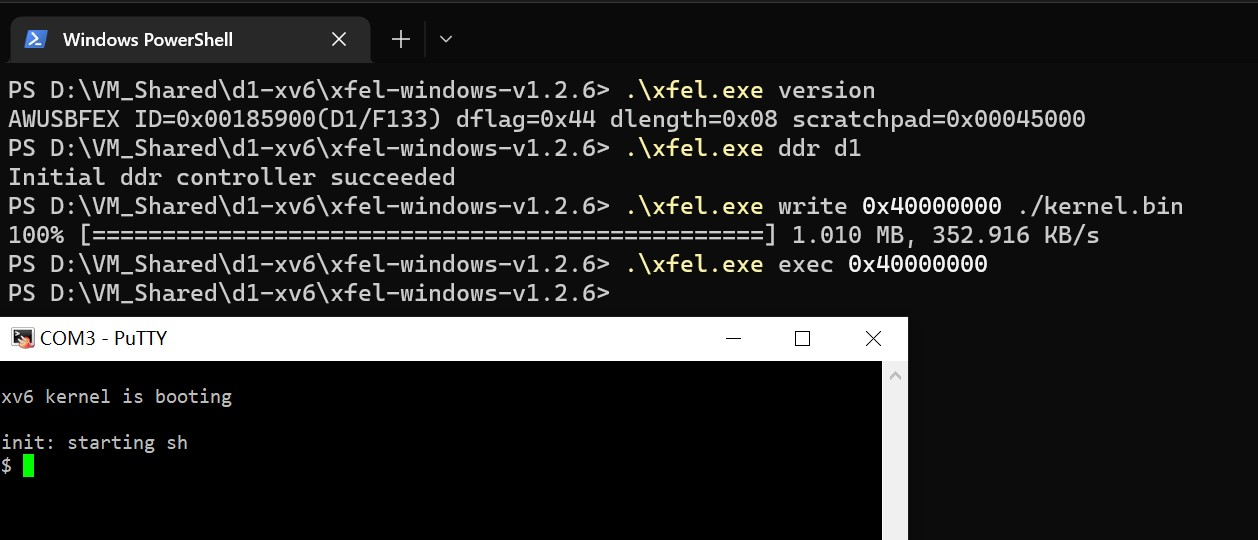
\includegraphics[width=0.7\textwidth]{RV_boot.jpg}
    \caption{ 在 Lichee RV 上启动 xv6}
\end{figure}

\begin{theorem}[Putty串口终端换行不正确]
    如果在连接开发板后,能够看到大概的输出,但是换行等格式较为混乱,则考虑在Putty的Terminal选项中勾选 Implicit CR in every LF 和 Implicit LF in every CR ,并将 Local echo 和 Local line editing 均设为 Force ,即可解决该问题。
\end{theorem}

可见在 Lichee RV 上成功启动 xv6 。下面尝试运行 \lstinline{usertests},结果如下图所示:

\begin{figure}[H]
    \centering
    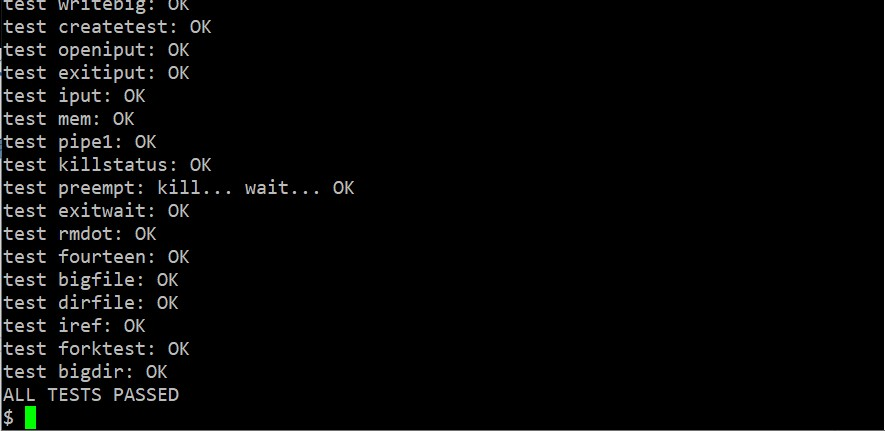
\includegraphics[width=0.7\textwidth]{RV_usertests.jpg}
    \caption{ 在 Lichee RV 上运行 \lstinline{usertests}}
\end{figure}

可见测试全部通过,说明我们在 Lichee RV 上运行 xv6 是成功的。

\section{给 xv6 增加一个应用编程语言}

能够在真实的硬件上跑 xv6 后,我们希望能够在 xv6 上提供给用户一个简易的开发环境,使其能够编写自己的用户态程序。由于类似 GCC 等工业级别的编译器的运行需要标准 C 语言库,而且其代码量巨大,移植较为困难,所以笔者选择了一种历史悠久、简单凝练但十分强大的语言 Scheme (一种 Lisp 方言\footnote{Lisp与Scheme的关系见:\url{https://en.wikipedia.org/wiki/Scheme_(programming_language)}第一段}),将其移植到原始的 xv6 环境中,从而使得 xv6 能成为可用的系统。

笔者选择移植的 Scheme 实现是由 Peter Michaux 实现的 Bootstrap Scheme\footnote{\url{https://github.com/petermichaux/bootstrap-scheme}}。 其本体仅由一个源文件构成,且依赖的标准 C 语言库中的内容十分少。

我们首先将其头文件更换为 xv6 提供的头文件:

\begin{lstlisting}[language=C]
// #include <stdlib.h>
// #include <stdio.h>
// #include <string.h>
// #include <ctype.h>

/**************************** FIXUP ******************************/
#include "kernel/types.h"
#include "user/user.h"
#include "kernel/fcntl.h"
#include <stdarg.h>
\end{lstlisting}

然后将输出的函数进行修改,以使其符合 xv6 用户C语言库的标准,在修改这些输出函数前,我们需要定义一些如\lstinline{stderr}的常量,以减少我们修改的工作量:
\begin{lstlisting}[language=C]
#define NULL 0
#define EOF 0
#define FD int

#define maxbufn 1024
#define maxfd 8

const int stdin = 0;
const int stdout = 1;
const int stderr = 2;
\end{lstlisting}

将所有的 \lstinline{fprintf}、\lstinline{open}、\lstinline{close} 等函数修改完成后,为了适应 xv6 中的 uart 串口中断,我们还需要实现几个常见的输入函数:
\begin{lstlisting}[language=C]

char ibuf[maxfd][maxbufn];
int bufptr[maxfd];
static char digits[] = "0123456789ABCDEF";

int getc(int fd)
{
  bufptr[fd]++;
  if (ibuf[fd][bufptr[fd]] == EOF || ibuf[fd][bufptr[fd]] == '\n' || ibuf[fd][bufptr[fd]] == '\r')
  {
    int i, cc;
    char c;
    bufptr[fd] = 0;
    for (i = 0; i + 1 < maxbufn;)
    {
      cc = read(fd, &c, 1);
      if (cc < 1)
        break;
      ibuf[fd][i++] = c;
      if (c == '\n' || c == '\r')
        break;
    }
  }
  int ret = ibuf[fd][bufptr[fd]];
  return ret;
}

void ungetc(char c, int fd)
{
  ibuf[fd][bufptr[fd]] = c;
  bufptr[fd]--;
}

void putc(char ch, int fd)
{
  ibuf[fd][++bufptr[fd]] = ch;
}

void fflush(int fd)
{
  ibuf[fd][++bufptr[fd]] = 0;
  fprintf(fd, ibuf[fd]);
  memset(ibuf[fd], 0x00, sizeof(ibuf[fd]));
  bufptr[fd] = 0;
}

void putchar(char c)
{
  printf("%c", c);
}

int isspace(char c) { return c == ' '; }
int isalpha(char c) { return (c >= 'a' && c <= 'z') || (c >= 'A' && c <= 'Z'); }
int isdigit(char c) { return (c >= '0' && c <= '9'); }
/**************************** MODEL ******************************/
\end{lstlisting}

将该源文件命名为 \lstinline{lisp.c} ,并将其加入到 Makefile 的用户程序中,继续修改细节直到通过编译。

\begin{theorem}[爆栈问题]
    通过编译后,在测试时发现,由于 xv6 的栈空间过小,故而导致其在使用递归函数时容易出现栈溢出的异常,进而修改 xv6 的 \lstinline{kernel/exec.c} 中的 \lstinline{exec()} 函数,增加其栈空间:
    \begin{lstlisting}[language=C]
        // Use the second as the user stack.
        int stack_pagenum = 1 + 1000;
        sz = PGROUNDUP(sz);
        uint64 sz1;
        if ((sz1 = uvmalloc(pagetable, sz, sz + stack_pagenum * PGSIZE)) == 0)
          goto bad;
        sz = sz1;
        uvmclear(pagetable, sz - stack_pagenum * PGSIZE);
        sp = sz;
        stackbase = sp - PGSIZE;
    \end{lstlisting}
    就可以缓解栈溢出的问题,要真正解决这个问题,需要在内核中实现栈内存动态分配的机制,相对较为繁琐。
\end{theorem}

进入 xv6 后,执行 \lstinline{lisp},就可以进入该编程语言的解释器,我们用如下的语句定义一个求 Fibonacci 数列的递归函数,然后试图求其第 15 项,如下图所示:

\begin{figure}[H]
    \centering
    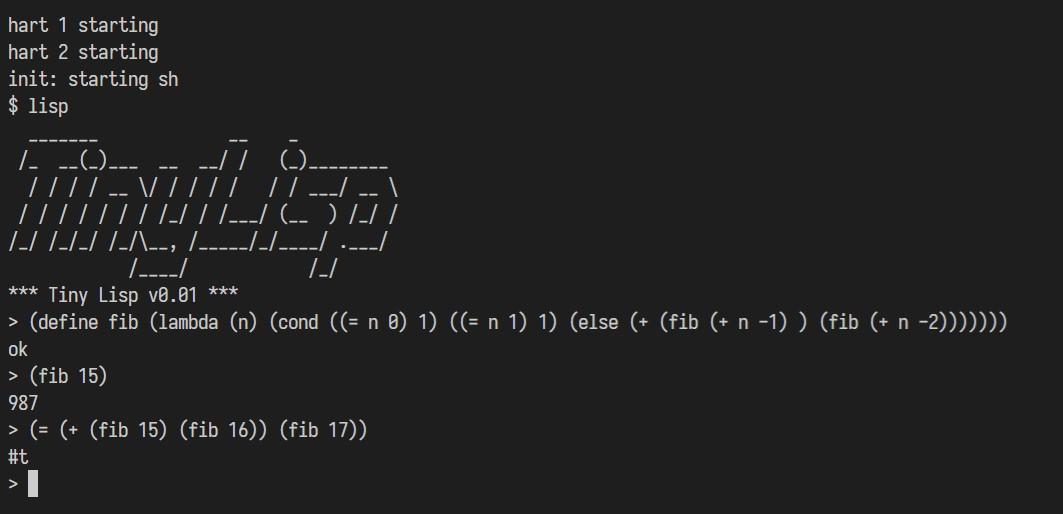
\includegraphics[width=0.7\textwidth]{RV_lisp.jpg}
    \caption{ 在 xv6 上使用 Scheme (Lisp) 编程求 Fibonacci 数列}
\end{figure}

可见程序运行符合预期,基本可以认为移植成功。

\section{更多后续的计划}

事实上,MIT 带给我们的 xv6 还有大量可以开发的潜力,下面列举笔者看到的一些比较有趣的关于 xv6 的开发计划:
\begin{enumerate}
    \item 使用 Rust 重写 xv6 (来自清华大学的项目)
    \item 将 xv6 移植到龙芯/MIPS架构上 (我校某同学的计划)
    \item 为 xv6 实现标准C语言库 (GitHub用户jahzielv的项目)
    \item 为 xv6 实现内核模块加载、卸载机制 (我校某同学的计划)
    \item 待续......
\end{enumerate}